\subsection{\label{sec:A23}p-dotiertes Silizium}
Im Vergleich zum hochohmigen Silizium wird ein THz-Puls aufgenommen, der durch einen Wafer aus 
p-dotierten Silizium (p-Si) propagiert. Die Aufnahmeparameter werden wie folgt gewählt
\begin{equation}
    \Delta s = 0,001\,\si{mm}, \hspace{1.5cm} N_{\text{s}} = 700, \hspace{1.5cm} N_{\text{sample}} = 100, \hspace{1.5cm} s_{0} = 153,3\,\si{mm},
\end{equation} 
was die schnelle Aufnahme des Hauptpulses ermöglicht. Der Aufgenommene Puls ist im Vergleich zum Referenzpuls in 
Abb.~\ref{fig:pdot} dargestellt. Es ist zu beachten, dass sich die Verzögerung $\Delta\tau$ auf zwei verschiedene 
Startpunkte bezieht, weswegen die gezeigten Pulse nur in ihrer Form und nicht in ihrer Position vergleichbar sind. \\ 
Im Unterschied zum HR-Si wird die Transmission beim Durchgang durch das p-Si mit dem Drude-Modell berechnet.
Grundlage hierfür ist die erhöhte Anzahl an freien Ladungsträgern, die mit dem THz-Feld 
wechselwirken und mit einer gedämpften Schwingung, der Plasma-Frequenz $\omega_{\text{p}}$ und 
Dämpfung $\Gamma$ reagieren. Für das HR-Si konnte diese Schwingung aufgrund der hohen 
Resistivität vernachlässigt werden. Es gelten folgende Zusammenhänge
\begin{align}
    T(\omega)_{\text{Drude}} &= \frac{4n(\omega)}{(n(\omega)+1)^{2}}e^{-i(n(\omega)-1)\omega L/c} \\
    n(\omega) &= \sqrt{\epsilon_{\infty} - \frac{\omega_{\text{p}}^{2}}{\omega^{2}-i\Gamma\omega}}.
\end{align}
Hierbei gibt $L$ die Dicke des 
Wafers an, für die wir $L = (380\pm5)\,\si{\mu m}$ messen 
(für den Fit wird der Wert als fehlerlos angenommen).
Die restlichen Größen sind als Konstanten definiert, 
wobei $\epsilon_{\infty}=3,4175^{2}$ und $m^{*} = 0,98m_{\text{elektron}}$
gilt \cite{Anleitung}.
Der theoretische Verlauf kann an die gemessene Transmission, 
welche analog zum vorherigen Abschnitt berechnet wird, 
über die Anpassung von $\omega_{\text{p}}$ und $\Gamma$ gefittet werden.
Hieraus lassen sich Materialeigenschaften wie die Ladungsträgermobilität $\mu$, 
die Ladungsträgerdichte $N$, die Leitfähigkeit $\sigma$ und der Widerstand 
$\rho = \sigma^{-1}$ berechnen.
\begin{figure}[h!]
    \centering
    \subfloat[\centering gemessene THz-Pulse]{{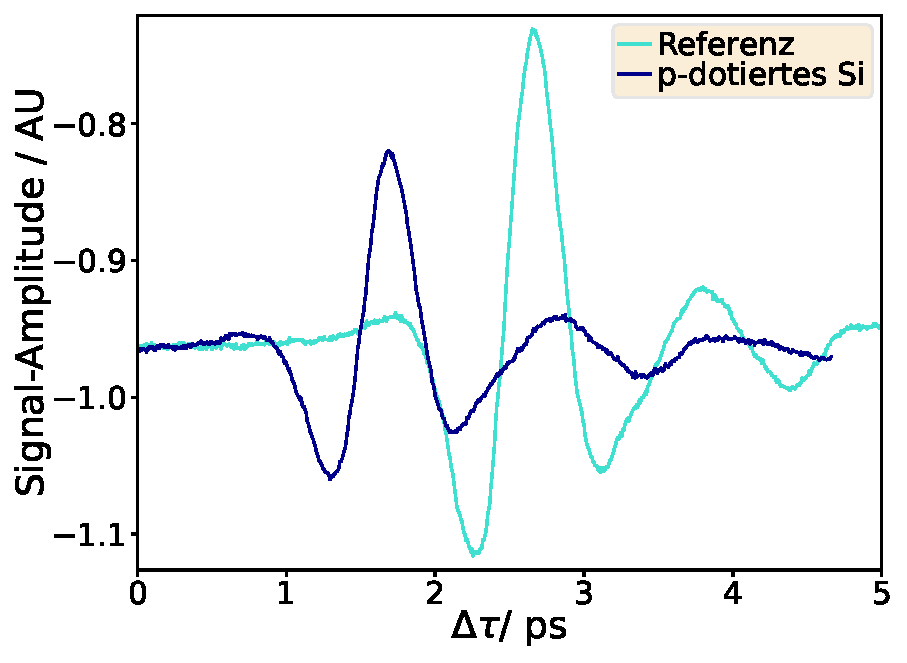
\includegraphics[width=0.47\textwidth]{pDotPuls.pdf} }}
    \qquad
    \subfloat[\centering Amplituden-Transmissionsspektrum]{{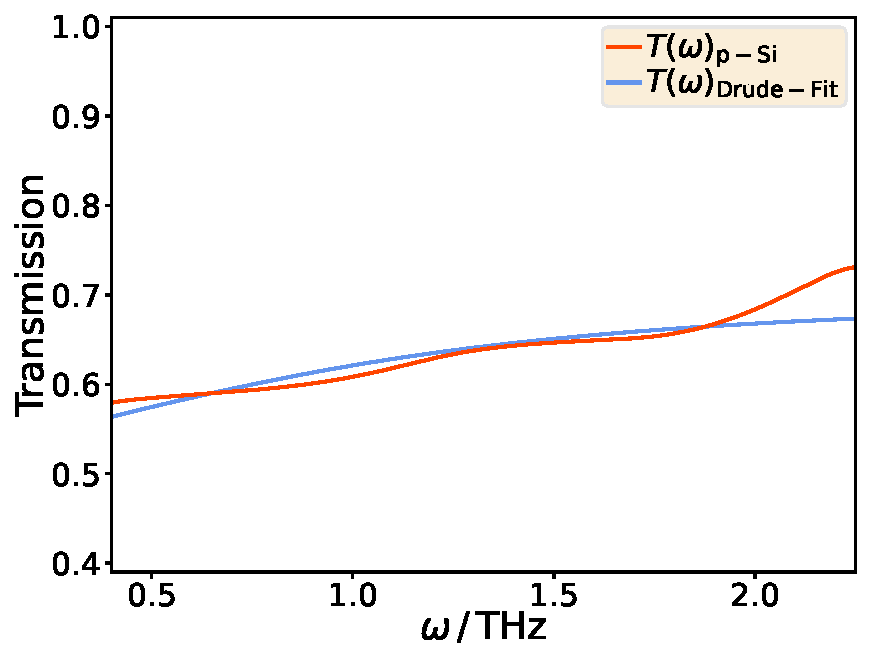
\includegraphics[width=0.47\textwidth]{pDotTrans.pdf} }}
    \caption{\label{fig:pdot}a) THz-Puls nach Propagation durch p-dotiertes Silizium (dunkelblau) im Vergleich
    mit dem Referenzpuls (hellblau). \\
    b) Das Amplituden-Transmissionsspektrum $T(\omega)$ für p-Si (orange) und die mit dem 
    Drude-Modell angefittete theoretische Transmission (hellblau).}
\end{figure}\FloatBarrier
Die Plasma-Frequenz und die Dämpfung der Schwingung erhalten wir aus dem in Python geschriebenen 
Fit-Programm, welches zusätzlich die Varianz der angepassten Werte liefert. 
Durch die Anwendung der Wurzel auf diese Größe ergibt sich der Fehler. Wir erhalten
\begin{equation}
    \fbox{$\omega_{\text{p}} = (1,45\pm 0,22)\,\si{THz} \hspace{2.5cm} \Gamma = (0,36\pm 0,17)\,\si{THz}$}.
\end{equation}
Hieraus lassen sich die erwähnten Materialparameter berechnen, für welche 
folgende Zusammenhänge gelten \cite{Anleitung}
\begin{alignat*}{2}
    \mu &= \frac{e}{m^{*}\Gamma} \quad \hspace{2.5cm}
    &&s_{\mu} = \frac{e}{m^{*}\Gamma^{2}}s_{\Gamma} \\
    N &= \frac{\omega_{\text{p}}^{2}m^{*}\epsilon_{\infty}\epsilon_{0}}{e^{2}}  \quad\hspace{2.5cm}
    &&s_{N} = 2\frac{\omega_{\text{p}}m^{*}\epsilon_{\infty}\epsilon_{0}}{e^{2}}s_{\omega_{\text{p}}} \\
    \sigma &= e\mu N \quad\hspace{2.5cm}
    &&s_{\sigma} = \sqrt{(eNs_{\mu})^{2} + (e\mu s_{N})^{2}} \\
    \rho &= \frac{1}{\sigma} \quad \hspace{2.5cm}
    &&s_{\rho} = \frac{1}{\sigma^{2}}s_{\sigma}.
\end{alignat*}
Mit den gefitteten Werten und der richtigen Umrechnung der SI-Einheiten in die üblichen zur 
Beschreibung verwendeten Einheiten folgt
\begin{alignat}{2}
    \Aboxed{\mu &= (1690 \pm 40)\,\si{\frac{cm^{2}}{Vs}} \hspace{2.5cm} N = (0,77 \pm 0,18)\cdot 10^{16}\,\si{\frac{1}{cm^{3}}}} \\
    \Aboxed{\sigma &= (2,08 \pm 0,7)\,\si{\frac{1}{\ohm cm}} \hspace{2.5cm} \rho = (0,48 \pm 0,15)\,\si{\ohm cm}}.
\end{alignat}
Die errechneten Werte liegen in einem sinnvollen Bereich für schwach p-dotiertes Silizium \cite{EPC}.
Es ist jedoch anzumerken, dass der von uns berechnete Widerstand unterhalb der unteren Grenze der 
Herstellerangabe liegt (Angabe $1-10\,\si{\ohm cm}$ \cite{Anleitung}). Da die Werte dennoch sinnvoll 
erscheinen und der Fit über eine andere Berechnungsmethode der spektralen Amplituden keine große 
Abweichung zeigt, gehen wir von der Richtigkeit der Messung aus. \\
Insgesamt können wir die THz-TDS auch erfolgreich auf p-dotiertes Silizium anwenden und 
das Spektrum an verwendeten Berechnungsmethoden erweitern. \\